\section{Correo Electrónico}

Hay tres protocolos principales para el correo electrónico, con distintos fines:

\begin{itemize}[label=\textcolor{acento}{$\bullet$}]
    \item \textbf{Distribución:} se utiliza el protocolo SMTP o Extended SMTP (ESMTP).
    \item \textbf{Entrega Final:} permite al usuario gestionar su correo a través de una máquina remota. Son POP3, IMAP o HTTP.
\end{itemize}

\begin{figure}[htbp]
    \centering
    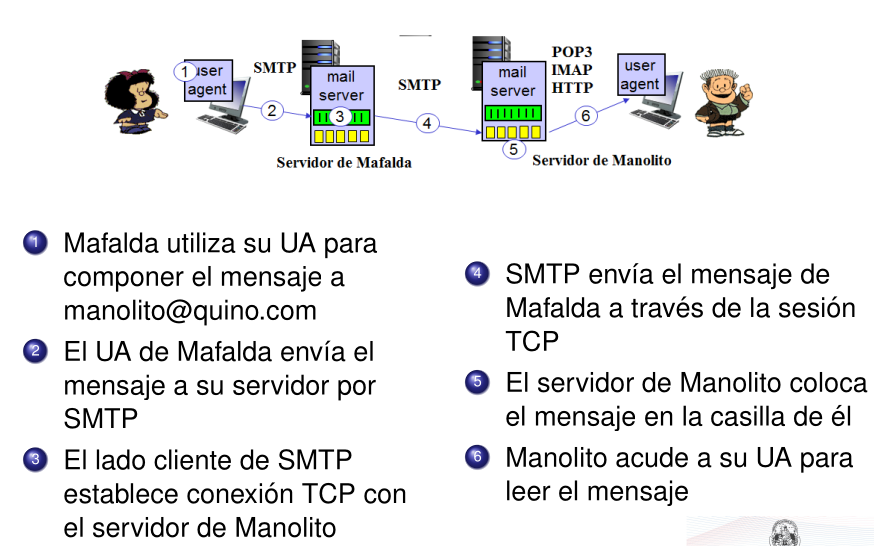
\includegraphics[width=0.8\textwidth]{capitulos/correo/imagenes/ciclo.png}
    \caption{Ciclo de un Correo Electrónico}
    \label{fig:ciclo-correo}
\end{figure}

\subsection{Simple Mail Transfer Protocol - SMTP}

\begin{definicion}{Definición}
    Tiene el objetivo de transferir mails de manera confiable y segura. El usuario coloca una copia del mensaje en el \emph{spool} y el cliente en \emph{background} envía los mensajes. El cliente barre los mensajes cada un cierto tiempo.  
\end{definicion}

Se utiliza DNS para resolver el nombre del destino en una dirección IP y luego se establece la conexión TCP con el servidor. 

\begin{enumerate}[label=\textcolor{acento}{\textbf{\arabic*.}}]
    \item El sender abre una conexión TCP al \textbf{puerto 25 del receptor}. 
    \item El \textbf{User Agent} consulta por el registro A de su servidor DNS.
    \item El \textbf{SMTP Server} hace una consulta DNS para obtener los registros \textbf{MX} del dominio destino. 
    \item Hacen un handshake entre el receptor y el emisor. 
\end{enumerate}

\subsubsection{Multipurpose Internet Mail Extensions - MIME}

\begin{definicion}{MIME}
    Es una extensión para enviar archivos ejecutables y multimedia mediante mail con ASCII de 7 bits, que era lo que permitía SMTP.
\end{definicion}


\subsection{Post Office Protocol 3 - POP3}

\begin{definicion}{POP3}
    Tiene como objetivo obtener el correo electrónico del buzón remoto y almacenarlo localmente en la PC del usuario para su lectura. Utiliza el \textbf{TCP en puerto 110}. 
\end{definicion}

Puede ser \emph{download and delete} o \emph{download and keep}. Según la modalidad borra o no los mensajes en la fase de actualización. En caso de que esté en \emph{download and delete}, no permite sincronismo entre otros dispositivos. 

\subsection{IMAP}

\begin{definicion}{IMAP}
    Asocia cada mensaje a una carpeta, sobre las cuales se pueden desplazar los mails. A diferencia de POP3, permite sincronismo entre otros dispositivos, ya que se accede al servidor para leer y no se borran los leídos.
    
    Funciona sobre \textbf{TCP en puerto 143}.
\end{definicion}

También incorpora descargas parciales de los mensajes. 